\documentclass[11pt,a4paper]{article}
\usepackage{ngerman}
\usepackage[ngerman]{babel}
\usepackage[utf8x]{inputenc}
\usepackage[T1]{fontenc}
\usepackage{lmodern}
\usepackage{marvosym}
\usepackage{amsfonts,amsmath,amssymb}
\usepackage{textcomp}
\usepackage{pifont}
\usepackage{ifpdf}
\usepackage[pdftex]{color}
\ifpdf
  \usepackage[pdftex]{graphicx}
\else
  \usepackage[dvips]{graphicx}\fi

\pagestyle{empty}

\usepackage[scale=0.775]{geometry}
\setlength{\parindent}{0pt}
\addtolength{\parskip}{6pt}

\def\firstname{Pascal}
\def\familyname{Bernhard}
\def\FileAuthor{\firstname~\familyname}
\def\FileTitle{\firstname~\familyname's Salz}
\def\FileSubject{Salz}
\def\FileKeyWords{\firstname~\familyname, Salz}

\renewcommand{\ttdefault}{pcr}
\hyphenation{ins-be-son-de-re}
\usepackage{url}
\urlstyle{tt}
\ifpdf
  \usepackage[pdftex,pdfborder=0,breaklinks,baseurl=http://,pdfpagemode=None,pdfstartview=XYZ,pdfstartpage=1]{hyperref}
  \hypersetup{
    pdfauthor   = \FileAuthor,%
    pdftitle    = \FileTitle,%
    pdfsubject  = \FileSubject,%
    pdfkeywords = \FileKeyWords,%
    pdfcreator  = \LaTeX,%
    pdfproducer = \LaTeX}
\else
  \usepackage[dvips]{hyperref}
\fi

\definecolor{firstnamecolor}{RGB}{56,115,179}
\definecolor{familynamecolor}{RGB}{56,115,179}
\hypersetup{pdfborder=0 0 0}

% Gleiche Schriftart für Hyperlinks
\urlstyle{same}


%  Gefrickel um URL-Links vernünftig umzubrechen
\makeatletter
\g@addto@macro\UrlBreaks{
  \do\a\do\b\do\c\do\d\do\e\do\f\do\g\do\h\do\i\do\j
  \do\k\do\l\do\m\do\n\do\o\do\p\do\q\do\r\do\s\do\t
  \do\u\do\v\do\w\do\x\do\y\do\z\do\&\do\1\do\2\do\3
  \do\4\do\5\do\6\do\7\do\8\do\9\do\0}
% \def\do@url@hyp{\do\-}

% Hiermit soll einer übervolle Box verhindert werden -- funktioniert sogar irgendwie
\g@addto@macro\UrlSpecials{\do\/{\mbox{\UrlFont/}\hskip 0pt plus 1pt}}
\makeatother

% Farben werden hier definiert
\definecolor{MidnightBlue}{RGB}{0,103,149}


\begin{document}
\sffamily   % for use with a résumé using sans serif fonts;
%\rmfamily  % for use with a résumé using serif fonts;
\hfill%
\begin{minipage}[t]{.6\textwidth}
\raggedleft%
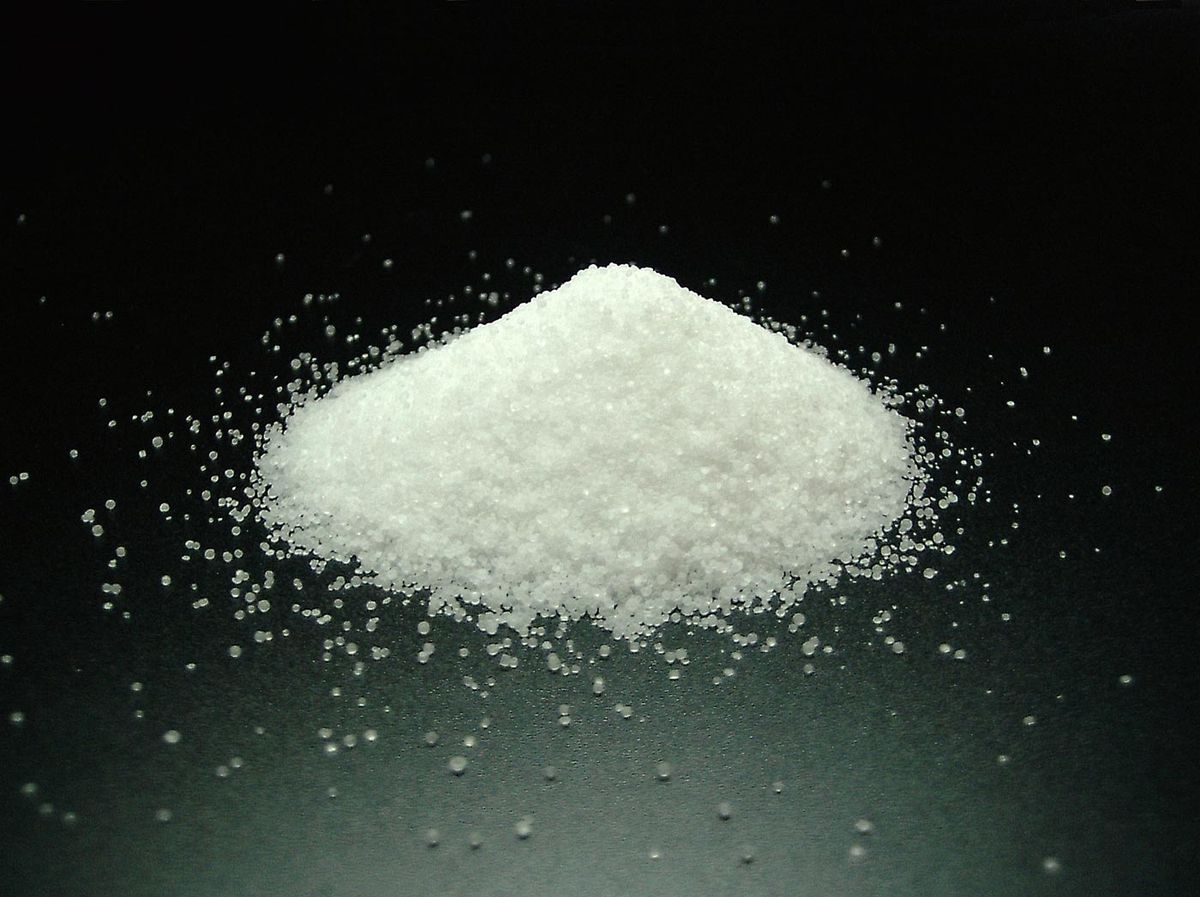
\includegraphics[width=0.55\textwidth]{Speisesalz.jpg}


\end{minipage}\\[0.5em]
%
{\color{firstnamecolor}\rule{\textwidth}{.25ex}}
%
\begin{minipage}[t]{.4\textwidth}
	\raggedright%
	% {\bfseries {\color{firstnamecolor}
	\vspace*{1em}
%	\textbf{Geschichte der Habsburger -- Flaggen} \\
%	 \\[.35ex]
	% }}
	\small%
%	Wolframstraße 89-92\\
%	12105 Berlin
\end{minipage}
%
\hfill
%
\begin{minipage}[t]{.4\textwidth}
	\raggedleft % US style
	\today
	%April 6, 2006 % US informal style
	%05/04/2006 % UK formal style
\end{minipage}\\[2.2em]


{\bfseries \color{familynamecolor}{{\LARGE Die Geschichte des Salzes}}}\\[0.75em]

\section*{\textsf{Die Bedeutung von Salz für die Menschen}}

\begin{itemize}
\item Salz (Natriumchlorid) ist für den menschlichen Körper unverzichtbar und somit ein wichtiger Bestandteil der Ernährung\\
\ding{225} Salz sorgt für die Regulierung des Wasser im Körper und ist für Muskeln und Knochen von Bedeutung

\item lange Zeit war Salz neben Alkohol und Räuchern eines der wenigen Mittel, Lebensmittel haltbar zu machen

\item bis zum 19. Jahrhundert war der Bedarf an Salz größer als die verfügbare Menge\\
\ding{225} Salz war so wertvoll, dass es auch als das '\textsl{weiße Gold}' bezeichnet wurde


\end{itemize}




\subsection*{\textsf{Salzhandel in der Antike}}

\begin{itemize}

\item bereits die Babylonier und Ägypter nutzten Salz zur Konservierung

\item seit der Steinzeit wird in Europa Salz in Bergwerken abgebaut, das älteste bekannte Salzbergwerk ist über 3000 Jahre alt und befindet sich in Hallstatt (Oberösterreich)\\
\ding{225} die Hallstättische Steinzeitkultur ist nach dem Ort der Salzgewinnung benannt

\item die Phönizier waren in der Antike (1200-900 vor Christus) die ersten, die Salz in großem Maßstab handelten\\
\ding{225} die lieferten Salz und Wein aus dem Mittelmeergebiet nach Nordeuropa und tauschten diese gegen Pelze, Bernstein und Zinn ein

\item die Kelten begann um 1000 v.Chr. mit dem Abbau von Salz in Bergwerken\\
\ding{225} \textsl{Hall} war das keltische Wort für Salz und bedeutet auch im Mittelhochdeutsch Salz (Bad Reichenhall, Hallstatt, Halle, Schwäbisch Hall, etc.)

\item im Mittelmeerraum wurde Salz in Meergärten durch Verdunstung von Meerwasser gewonnen

\item im Römischen Reich existierte ein 'Salzverteilernetz' aus spezialisierten Kaufleuten, den \textsl{salarii}, die Salz bis in die entlegendsten Regionen des Reiches transportierten\\
\ding{225} dieses Salznetz funktionierte so reibungslos, dass der Preis für das Gut im Vergleich zum Mittelalter sehr stabil war


\item diese Preisstabilität und die geregelte Versorgung ermöglichte es den Römern, Salz als Zahlungsmittel zu verwenden\\
\ding{225} die römischen Legionäre erhielten ihr Gehalt im Form von Salz, das sog. \textsl{salarium} (salary, salaire, Salär)


\item der Verkauf von Salz (wie auch von Waffen und Getreide) an die Feinde des Römischen Reiches war streng verboten


\end{itemize}



\subsection*{\textsf{Salz im Mittelalter Europas}}

\begin{itemize}

\item mit dem Niedergang und Ende des Römischen Reiches kam der europäische Salzhandel zum Erliegen\\
\ding{225} Salz musste lokal gewonnen werden, z.B. in sogenannten \textsl{Solen}

	\begin{itemize}
	\item in Solen wird mit Salz gesättigtes Wasser durch Verheizen von Brennholz verdampft, das Salz bleibt zurück
	\item der große Bedarf an Brennholz hat zum Entstehen der Heidelandschaft um Lüneburg beigetragen\\
	\ding{225} keine nachhaltige Form der Salzgewinnung
	\end{itemize}

\item Salzhandel über lange Distanzen war im mittelalterlichen Europa nicht mehr möglich, so dass nicht mehr das günstigere Meersalz aus der Mittelmeerregion verwendet wurde\\
\ding{225} die Salzbergwerke im Alpenraum erlebten einen Wiederaufschwung

\item die Salzkaufleute benutzten nur Straßen, die unter dem Schutz von adeligen Herren standen, da andere Transportwege zu gefährlich waren\\
\ding{225} diese Herren erhoben Steuern auf Transport und das Salz selbst

	\begin{itemize}
	\item die Salzsteuern wurden zu einer sprudelnden Einnahmequelle für Fürsten und an Salzstraßen gelegenen Städte\\
	\ding{225} der französische König erhob die '\textsl{gabelle}' genannte Salzsteuer\\
	\ding{225} von Philipp IV im Jahre 1286 als Notmaßnahme eingeführt wurde die \textsl{gabelle} im 14. Jahrhundert zu einer fortwährenden Abgabe\\
	\ding{225} alle Personen über 8 Jahre mussten wöchentlich ein Mindestmenge an Salz zu einem festgesetzten Preis kaufen
	
	\item wichtige Städte, die durch den Salzhandel zu Größe und Wohlstand kamen: Rom, München, Lüneburg, Warschau, die Hansestädte, aber auch Timbuktu in Afrika
	
	\item da Salz unverzichtbar war und die Salzsteuern schwer zu umgehen, stieg der Preis des Salz stetig\\
	\ding{225} bis zum 16. Jahrhundert war Salz als Gewürz (nicht zu verwechseln mit der Verwendung als Konservierungsmittel) nur an Fürstenhöfen und reichen Händlerfamilien zu finden -- die einfachen Leute verwendeten Pflanzenasche als Salzersatz
	\end{itemize}

\item große Bedeutung im Mittelalter hatte die 'alte Salzstraße' von Halle, über Leipzig und das Erzgebirge nach Prag, da es in Böhmen keine Salzvorkommen gab

\item im Mittelalter wurde Salz auch bei Verarbeitung von Fellen, der Veredelung von Metallen (für Waffen und Werkzeuge) und der Herstellung von Keramik und Glas gebraucht


\end{itemize}


\subsection*{\textsf{Neuzeit}}

\begin{itemize}

\item mit der Herausbildung von Nationalstaaten zusammen mit der Entwicklung effektiver Verwaltungsstrukturen wurde die Salzsteuer als eine Verbrauchsteuer zum Monopol der Staaten\\
\ding{225} die Salzsteuer war Grundpfeiler der staatlichen Finanzen

\item ständig steigende Steuern führten zu Unruhen in der Bevölkerung, wie zum Beispiel in Frankreich gegen die \textsl{gabelle}

\item die Techniken des Salzabbaus in Bergwerken entwickelte sich ab dem frühen 17. Jahrhundert weiter, so dass die Produktion gesteigert werden konnte\\
\ding{225} allmählich fiel der Salzpreis und auch die einfache Bevölkerung konnte sich Salz als Gewürz für Speisen leisten

	\begin{enumerate}
	\item in 1616 wurde in Bad Reichenhall erstmals ein Pumpensystem zum Abpumpen des Wasser eingesetzt
	\item mit Dampfmaschinen betriebene Pumpen brachten die Salzproduktion einem industriellen Niveau näher
	\item um 1850 begann in Deutschland der 'bergmännische Abbau' von Salz in Bergwerken\\
	\ding{225} es war möglich geworden, Salzvorkommen wurden wissenschaftliche lokalisiert
	\end{enumerate}

\item mit der industriellen Produktion von Salz und dem allgemeinen wirtschaftlichen Aufstieg Europa verlor die Besteuerung von Salz als Einnahmequelle des Staates an Bedeutung\\
\ding{225} Steuermonopole auf Salz fielen Anfang des 20. Jahrhunderts weg

\item in Deutschland werden heute 12.5 Mio. Tonnen Salz pro Jahr gewonnen, das entspricht 7 \% der Weltproduktion

\item nur noch 3 \% das Salzgewinnung wird heutzutage für die menschliche Ernährung benötigt, der größte Teil kommt bei der Herstellung von Glas, Chlor und dem Färben von Textilien zum Einsatz

\end{itemize}


\end{document}